\chapter{Introduction and Asymptotic Analysis for Tukey Depth in the Bivariate Exponential Distribution}

\section{Introduction}

In this chapter, we study the Tukey (half-space) depth for a bivariate distribution with independent exponential marginals. Let
\[
X \sim \operatorname{Exp}(\lambda_1) \quad\text{and}\quad Y \sim \operatorname{Exp}(\lambda_2),
\]
with joint density
\[
f_{X,Y}(x,y)=\lambda_1\lambda_2 \, e^{-\lambda_1 x-\lambda_2 y},\quad x,y \ge 0.
\]
The Tukey depth of a point is traditionally defined as the minimum probability mass of any closed half-space that contains the point. In our analysis, rather than simply comparing the probability mass \(P\) on one side of a fixed line with \(1-P\), we consider a family of lines (or equivalently, directions) passing through the point \((a,b)\) and study the probability mass on one side of each line. Although one may be tempted to express the depth as
\[
D(a,b)=\min\{P,1-P\},
\]
this formulation is not a complete definition of Tukey depth. First, it applies only for a given direction; the full depth is obtained by taking the infimum over all directions. Second, while for points with large coordinates (i.e. \(x \gg 0\) and \(y \gg 0\)) one side of the half-space tends to dominate, for points near the origin the “inner” probability (the mass on the side closer to the high-density region) can actually be lower than the “outer” probability. Hence, one cannot simply compute \(1-P\) and then take the minimum; the correct notion of depth requires a careful examination of the probability mass as a function of the line parameters and then taking the infimum over all admissible directions.


\section{Definition of the Probability Mass \( I(k) \)}

Consider a line through \((a,b)\) given by
\begin{equation}\label{eq:line}
  y - b = k\,(x - a),
\end{equation}
with \(k = \tan\theta\). In the first quadrant (\(x\ge0,\, y\ge0\)), the half-space defined by this line generally leads to different integration regions depending on where the line crosses the axes. Figure~\ref{fig:regions} illustrates three cases:

\begin{description}
  \item[\textbf{Case I (Triangle):}] Both the \(x\)- and \(y\)-intercepts are positive. In this case, the line crosses the \(x\)-axis at
  \[
  x_0 = a - \frac{b}{k} > 0,
  \]
  and the \(y\)-axis at
  \[
  y_0 = b - ka > 0.
  \]
  Hence, for \(x\in[0,x_0]\) the integration in \(y\) runs from \(0\) up to 
  \[
  y_{\max}(x)=k(x-a)+b,
  \]
  and the region is the simple triangle formed by the line and the axes.

  \item[\textbf{Case II (Negative \(x\)-intercept, Positive \(y\)-intercept):}] If the \(x\)-intercept is negative, i.e.,
  \[
  x_0 = a - \frac{b}{k} < 0,
  \]
  while the \(y\)-intercept remains positive, then the region in the first quadrant is defined by \(x\ge0\) and \(y\in\bigl[0,\,k(x-a)+b\bigr]\).

  \item[\textbf{Case III (Positive \(x\)-intercept, Negative \(y\)-intercept):}] If the line crosses the \(y\)-axis in the negative region,
  \[
  y_0 = b - ka < 0,
  \]
  while \(x_0 = a - \frac{b}{k} > 0\), then the boundary relevant in the first quadrant starts at \(x=x_0\) (since for \(x<x_0\) the line lies below \(y=0\)) and extends for \(x\ge x_0\) with \(y\) between 0 and \(k(x-a)+b\).
\end{description}

\begin{figure}[h]
  \centering
  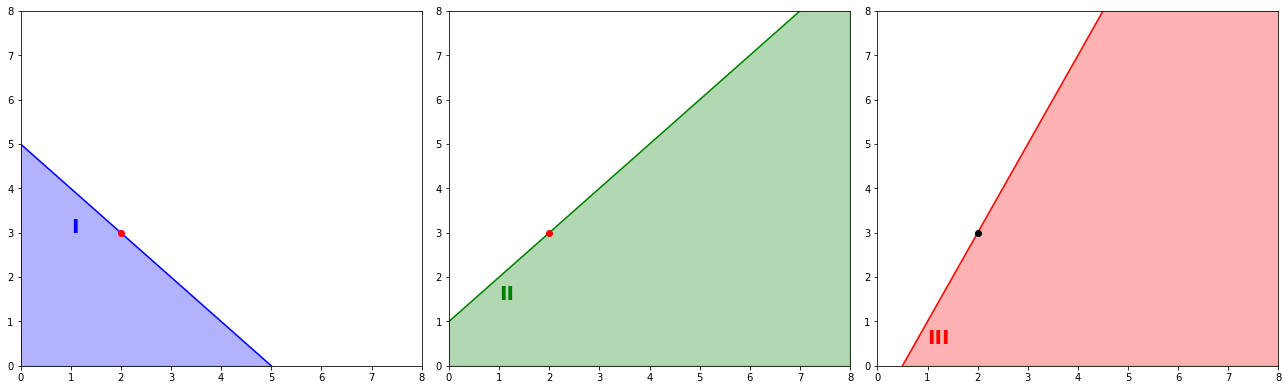
\includegraphics[width=1.0\textwidth]{images/picture1.png}
  \caption{Visualization of Regions Defined by Lines Through \((a,b)\): Case I shows the triangular region (both intercepts positive), Case II the region when the \(x\)-intercept is negative, and Case III when the \(y\)-intercept is negative.}
  \label{fig:regions}
\end{figure}

In fact, Cases II and III can be grouped together. In these cases, the integration region in the first quadrant is given by
\[
  x \ge \max\{0,x_0\} \quad \text{and} \quad 0\le y \le k(x-a)+b.
\]
Thus, a unified expression for the probability mass below the line is
\begin{equation}\label{eq:Ik_general}
  I(k)=\int_{x=\max\{0,x_0\}}^{\infty} \int_{y=0}^{k(x-a)+b} \lambda_1 \lambda_2 \, e^{-\lambda_1 x-\lambda_2 y} \, dy\,dx,
\end{equation}
with the understanding that in Case I (the triangle) the integration naturally runs over \(x\in[0,x_0]\).

\section{Analytical Computation of \( I(k) \)}

To identify the optimal slope \( k^* \) minimizing the half-space probability mass, we need to differentiate \( I(k) \) with respect to \( k \) and solve \( dI/dk=0 \). As discussed, the integration domain depends on the intercepts, so we consider the two scenarios separately.

\subsection*{Case I (Triangle Region)}

When both intercepts are positive the integration region is 
\[
x\in\left[0,x_0\right],\quad \text{with}\quad x_0=a-\frac{b}{k}>0.
\]
In this case, the probability mass is given by
\begin{equation}\label{eq:Ik_case1}
  I_1(k)=\int_{0}^{x_0} \lambda_1 e^{-\lambda_1 x}\left[ 1-e^{-\lambda_2\bigl(k(x-a)+b\bigr)} \right]dx.
\end{equation}
This integral can be computed in closed form. In fact, writing
\[
I_1(k)=\underbrace{\int_{0}^{x_0} \lambda_1 e^{-\lambda_1 x}\,dx}_{=1-e^{-\lambda_1x_0}} - \underbrace{\int_{0}^{x_0} \lambda_1 e^{-\lambda_1 x}e^{-\lambda_2\bigl(k(x-a)+b\bigr)}dx}_{:=J(k)},
\]
we note that
\[
J(k)=e^{-\lambda_2(ka-b)}\int_{0}^{x_0} \lambda_1 e^{-(\lambda_1+\lambda_2k)x}\,dx 
= e^{-\lambda_2(ka-b)}\,\frac{\lambda_1}{\lambda_1+\lambda_2k}\left[1-e^{-(\lambda_1+\lambda_2k)x_0}\right].
\]
Thus, we obtain
\[
I_1(k)=\left[1-e^{-\lambda_1\left(a-\frac{b}{k}\right)}\right] - e^{-\lambda_2(ka-b)}\,\frac{\lambda_1}{\lambda_1+\lambda_2k}\left[1-e^{-(\lambda_1+\lambda_2k)\left(a-\frac{b}{k}\right)}\right].
\]
This expression, though somewhat involved, is fully analytical and can be differentiated with respect to \( k \) using standard calculus rules.

\subsection*{Cases II+III (Grouped Region)}

When one of the intercepts is non-positive, the integration region in the first quadrant becomes
\[
x \ge \max\{0,x_0\}, \quad \text{with}\quad x_0 = a-\frac{b}{k}.
\]
Define
\[
A = \max\Bigl\{0,\,a-\frac{b}{k}\Bigr\}.
\]
Then, the probability mass is given by
\begin{equation}\label{eq:Ik_case23}
  I_2(k)=\int_{A}^{\infty} \lambda_1 e^{-\lambda_1 x}\Bigl[1-e^{-\lambda_2\bigl(k(x-a)+b\bigr)}\Bigr]dx.
\end{equation}
As in Case I, we split the integral:
\[
I_2(k)=\left[\int_{A}^{\infty} \lambda_1 e^{-\lambda_1 x}dx\right]-\left[\int_{A}^{\infty} \lambda_1 e^{-\lambda_1 x}e^{-\lambda_2\bigl(k(x-a)+b\bigr)}dx\right].
\]
The first term is elementary:
\[
\int_{A}^{\infty} \lambda_1 e^{-\lambda_1 x}dx = e^{-\lambda_1 A}.
\]
For the second term, we rewrite
\[
e^{-\lambda_2\bigl(k(x-a)+b\bigr)} = e^{-\lambda_2k(x-a)}\,e^{-\lambda_2b} = e^{\lambda_2ka-\lambda_2b}\,e^{-\lambda_2kx}.
\]
Thus,
\[
\int_{A}^{\infty} \lambda_1 e^{-\lambda_1 x}e^{-\lambda_2\bigl(k(x-a)+b\bigr)}dx = e^{\lambda_2ka-\lambda_2b}\int_{A}^{\infty} \lambda_1 e^{-(\lambda_1+\lambda_2k)x}dx.
\]
Evaluating the remaining integral, we have
\[
\int_{A}^{\infty} \lambda_1 e^{-(\lambda_1+\lambda_2k)x}dx = \frac{\lambda_1}{\lambda_1+\lambda_2k}\,e^{-(\lambda_1+\lambda_2k)A}.
\]
Therefore, the closed-form expression for \(I_2(k)\) is
\[
I_2(k)=e^{-\lambda_1 A} - \frac{\lambda_1}{\lambda_1+\lambda_2k}\,e^{\lambda_2ka-\lambda_2b-(\lambda_1+\lambda_2k)A}.
\]
This expression can be rewritten as
\[
I_2(k)=e^{-\lambda_1 A}\left[1-\frac{\lambda_1}{\lambda_1+\lambda_2k}\,e^{\lambda_2k(a-A)-\lambda_2b}\right],
\]
with
\[
A=\max\left\{0,\,a-\frac{b}{k}\right\}.
\]

\section{Asymptotic Behaviour: Small-Scale Regime}

In the small-scale regime the closed-form expressions for the probability mass corresponding to a half-space defined by a line through \((a,b)\) simplify considerably. Recall that we derived
\[
I_1(k)=\Bigl[1-e^{-\lambda_1\Bigl(a-\frac{b}{k}\Bigr)}\Bigr]
- e^{-\lambda_2(ka-b)}\,\frac{\lambda_1}{\lambda_1+\lambda_2k}\Bigl[1-e^{-(\lambda_1+\lambda_2k)\Bigl(a-\frac{b}{k}\Bigr)}\Bigr],
\]
for the triangular region (where both intercepts are positive, with integration over
\[
x\in\Bigl[0,a-\frac{b}{k}\Bigr],
\]
and
\[
I_2(k)=e^{-\lambda_1A}\Biggl[1-\frac{\lambda_1}{\lambda_1+\lambda_2k}\,e^{\lambda_2k(a-A)-\lambda_2b}\Biggr],
\]
for the grouped region (where at least one intercept is non-positive, with
\[
x\in\Bigl[\max\Bigl\{0,a-\frac{b}{k}\Bigr\},\infty\Bigr),
\]
and we define
\[
A=\max\Bigl\{0,\,a-\frac{b}{k}\Bigr\}.
\]

In our small-scale analysis we assume that the argument
\[
g(x)=k(x-a)+b
\]
remains sufficiently small so that a first-order Taylor expansion is valid. With the standard expansion
\[
e^{-z}\approx 1-z,
\]
we expand the exponentials in the above expressions. After some algebra, one finds that the optimal slope (minimizing the half-space measure) satisfies
\[
k^*\approx\frac{\lambda_1}{\lambda_2}\quad \text{or equivalently}\quad \tan\theta^*\approx\frac{\lambda_1}{\lambda_2}.
\]

Assuming that
\[
a-\frac{b\lambda_2}{\lambda_1}>0,
\]
we then have, for the grouped region, an effective lower integration limit
\[
A^*=a-\frac{b\lambda_2}{\lambda_1}.
\]
Under this condition the algebra shows that the expression corresponding to the grouped region becomes asymptotically lower. In particular, substituting \(k^*=\lambda_1/\lambda_2\) yields
\[
I_2(k^*)\approx \frac{1}{2}\,e^{-\lambda_1\Bigl(a-\frac{b\lambda_2}{\lambda_1}\Bigr)}.
\]
Thus, in the regime where
\[
a-\frac{b\lambda_2}{\lambda_1}>0,
\]
the infimum over the half-space measures (i.e. the Tukey depth) is asymptotically approximated by the value obtained in the grouped region.

\section{Summary}

In this chapter we developed an analytical framework for approximating the infimum of the half-space measure for a bivariate exponential distribution. We derived closed-form expressions for the probability mass \(I(k)\) associated with half-spaces defined by lines through \((a,b)\) in two cases:
\begin{itemize}
    \item \textbf{Case I (Triangular Region):} When both intercepts are positive, with integration over
    \[
    x\in\Bigl[0,a-\frac{b}{k}\Bigr],
    \]
    \item \textbf{Cases II+III (Grouped Region):} When at least one intercept is non-positive, with integration over
    \[
    x\in\Bigl[\max\Bigl\{0,a-\frac{b}{k}\Bigr\},\infty\Bigr).
    \]
\end{itemize}

Focusing on the small-scale regime (i.e. when \(g(x)=k(x-a)+b\) is small) and applying a first-order Taylor expansion, we found that the optimal slope satisfies
\[
k^*\approx\frac{\lambda_1}{\lambda_2}\quad (\tan\theta^*\approx\lambda_1/\lambda_2).
\]
Assuming further that
\[
a-\frac{b\lambda_2}{\lambda_1}>0,
\]
the analysis shows that the half-space corresponding to the grouped region provides the lower measure, and its value is asymptotically given by
\[
I_2(k^*)\approx \frac{1}{2}\,e^{-\lambda_1\Bigl(a-\frac{b\lambda_2}{\lambda_1}\Bigr)}.
\]
This expression represents the infimum over all half-spaces (and hence the Tukey depth) in the considered regime. Future work will address the complementary case where
\[
a-\frac{b\lambda_2}{\lambda_1}\le 0,
\]
and will compare these asymptotic predictions with full numerical evaluations.
